\documentclass[dvipsnames, tikz]{standalone}
\usepackage{amsmath}
\usepackage{arevmath}
\usepackage{xcolor}
\usepackage{tikz}
\usetikzlibrary{calc}
\usetikzlibrary{decorations.pathreplacing,calligraphy,3d}
\usetikzlibrary{matrix,shapes,fit,backgrounds}

\tikzset{%Global config
	>=latex,
	color = black ,
	%Styles
	Matrix/.style={
		matrix of nodes,
		line width=1pt,
		text height=1.75ex,
		%text depth=0.75ex,
		text width=2.25ex,
		align=center,
		column sep=1pt,
		row sep=1pt,
		nodes={draw=black!10}, % Uncoment to see the square nodes.
		nodes in empty cells,
	},
	DA/.style={
		fill,
		opacity=0.3,
		%rounded corners,
		inner sep=0pt,
		line width=1pt,
	},
	DG/.style={
		line cap = round,
		rounded corners=0.25ex,
		line width = 10pt,
		opacity = 0.3,
	}
	]
}

\begin{document}
	\begin{tikzpicture}
		\clip (0,0) rectangle(2.8,-2.5);
		\matrix[Matrix, anchor=north west] at (0,0) (M){ % Matrix contents  
			\sf  1 \\
		};
	\end{tikzpicture}
	
	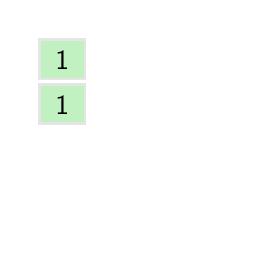
\begin{tikzpicture}
		\clip (0,0) rectangle(2.8,-2.5);
		\matrix[Matrix, anchor=north west] at (0,0) (M){ % Matrix contents  
			\sf 1 \\
			\sf 1\\
		};
	
		\begin{scope}[on background layer] 
			\node[DA,LimeGreen,fit=(M-1-1)(M-1-1)](subM){};
			\node[DA,LimeGreen,fit=(M-2-1)(M-2-1)](subM){};
		\end{scope}
	\end{tikzpicture}

		\begin{tikzpicture}
		\clip (0,0) rectangle(2.8,-2.5);
		\matrix[Matrix, anchor=north west] at (0,0) (M){ % Matrix contents  
			\sf 1 \\
			\sf 1\\
		};
	\end{tikzpicture}

	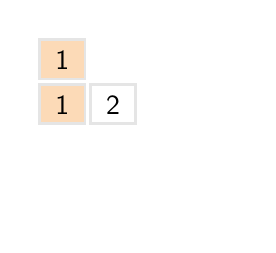
\begin{tikzpicture}
		\clip (0,0) rectangle(2.8,-2.5);
		\matrix[Matrix, anchor=north west] at (0,0) (M){ % Matrix contents  
			\sf 1 \\
			\sf 1 & \sf 2\\
		};
		
		\begin{scope}[on background layer] 
			\node[DA,BurntOrange,fit=(M-1-1)(M-1-1)](subM){};
			\node[DA,BurntOrange,fit=(M-2-1)(M-2-1)](subM){};
		\end{scope}
	\end{tikzpicture}

	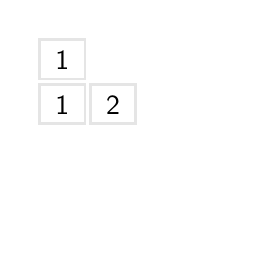
\begin{tikzpicture}
		\clip (0,0) rectangle(2.8,-2.5);
		\matrix[Matrix, anchor=north west] at (0,0) (M){ % Matrix contents  
			\sf 1 \\
			\sf 1 & \sf 2\\
		};
	\end{tikzpicture}

	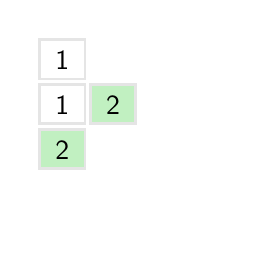
\begin{tikzpicture}
		\clip (0,0) rectangle(2.8,-2.5);
		\matrix[Matrix, anchor=north west] at (0,0) (M){ % Matrix contents  
			\sf 1 \\
			\sf 1 & \sf 2\\
			\sf 2 \\
		};
		
		\begin{scope}[on background layer] 
			\node[DA,LimeGreen,fit=(M-2-2)(M-2-2)](subM){};
			\node[DA,LimeGreen,fit=(M-3-1)(M-3-1)](subM){};
		\end{scope}
	\end{tikzpicture}

	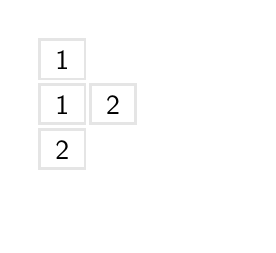
\begin{tikzpicture}
		\clip (0,0) rectangle(2.8,-2.5);
		\matrix[Matrix, anchor=north west] at (0,0) (M){ % Matrix contents  
			\sf 1 \\
			\sf 1 & \sf 2\\
			\sf 2 \\
		};
		
		\begin{scope}[on background layer] 
			%\node[DA,LimeGreen,fit=(M-2-2)(M-2-2)](subM){};
			%\node[DA,LimeGreen,fit=(M-3-1)(M-3-1)](subM){};
		\end{scope}
	\end{tikzpicture}

	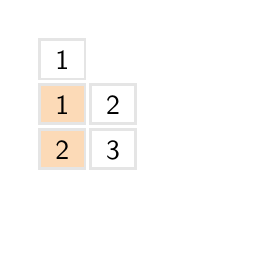
\begin{tikzpicture}
		\clip (0,0) rectangle(2.8,-2.5);
		\matrix[Matrix, anchor=north west] at (0,0) (M){ % Matrix contents  
			\sf 1 \\
			\sf 1 & \sf 2\\
			\sf 2 & \sf 3\\
		};
		
		\begin{scope}[on background layer] 
			\node[DA,BurntOrange,fit=(M-2-1)(M-2-1)](subM){};
			\node[DA,BurntOrange,fit=(M-3-1)(M-3-1)](subM){};
		\end{scope}
	\end{tikzpicture}

	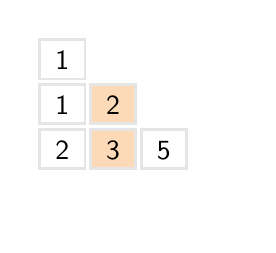
\begin{tikzpicture}
		\clip (0,0) rectangle(2.8,-2.5);
		\matrix[Matrix, anchor=north west] at (0,0) (M){ % Matrix contents  
			\sf 1 \\
			\sf 1 & \sf 2\\
			\sf 2 & \sf 3 & \sf 5\\
		};
		
		\begin{scope}[on background layer] 
			\node[DA,BurntOrange,fit=(M-2-2)(M-2-2)](subM){};
			\node[DA,BurntOrange,fit=(M-3-2)(M-3-2)](subM){};
		\end{scope}
	\end{tikzpicture}

	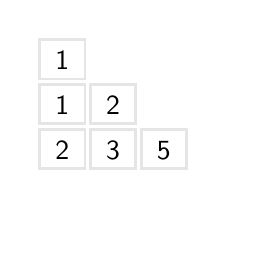
\begin{tikzpicture}
		\clip (0,0) rectangle(2.8,-2.5);
		\matrix[Matrix, anchor=north west] at (0,0) (M){ % Matrix contents  
			\sf 1 \\
			\sf 1 & \sf 2\\
			\sf 2 & \sf 3 & \sf 5\\
		};
		
		\begin{scope}[on background layer] 
			%\node[DA,BurntOrange,fit=(M-2-2)(M-2-2)](subM){};
			%\node[DA,BurntOrange,fit=(M-3-2)(M-3-2)](subM){};
		\end{scope}
	\end{tikzpicture}

	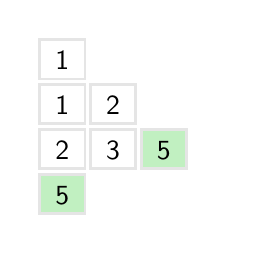
\begin{tikzpicture}
		\clip (0,0) rectangle(2.8,-2.5);
		\matrix[Matrix, anchor=north west] at (0,0) (M){ % Matrix contents  
			\sf 1 \\
			\sf 1 & \sf 2\\
			\sf 2 & \sf 3 & \sf 5\\
			\sf 5\\
		};
		
		\begin{scope}[on background layer] 
			\node[DA,LimeGreen,fit=(M-3-3)(M-3-3)](subM){};
			\node[DA,LimeGreen,fit=(M-4-1)(M-4-1)](subM){};
		\end{scope}
	\end{tikzpicture}

	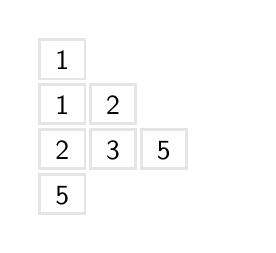
\begin{tikzpicture}
		\clip (0,0) rectangle(2.8,-2.5);
		\matrix[Matrix, anchor=north west] at (0,0) (M){ % Matrix contents  
			\sf 1 \\
			\sf 1 & \sf 2\\
			\sf 2 & \sf 3 & \sf 5\\
			\sf 5\\
		};
	\end{tikzpicture}

	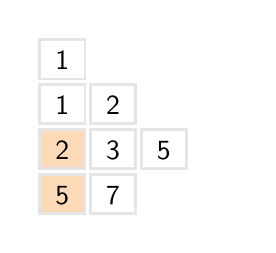
\begin{tikzpicture}
		\clip (0,0) rectangle(2.8,-2.5);
		\matrix[Matrix, anchor=north west] at (0,0) (M){ % Matrix contents  
			\sf 1 \\
			\sf 1 & \sf 2\\
			\sf 2 & \sf 3 & \sf 5\\
			\sf 5 & \sf 7\\
		};
		
		\begin{scope}[on background layer] 
			\node[DA,BurntOrange,fit=(M-3-1)(M-3-1)](subM){};
			\node[DA,BurntOrange,fit=(M-4-1)(M-4-1)](subM){};
		\end{scope}
	\end{tikzpicture}

	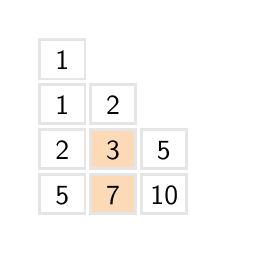
\begin{tikzpicture}
		\clip (0,0) rectangle(2.8,-2.5);
		\matrix[Matrix, anchor=north west] at (0,0) (M){ % Matrix contents  
			\sf 1 \\
			\sf 1 & \sf 2\\
			\sf 2 & \sf 3 & \sf 5\\
			\sf 5 & \sf 7 & \sf 10\\
		};
		
		\begin{scope}[on background layer] 
			\node[DA,BurntOrange,fit=(M-3-2)(M-3-2)](subM){};
			\node[DA,BurntOrange,fit=(M-4-2)(M-4-2)](subM){};
		\end{scope}
	\end{tikzpicture}

	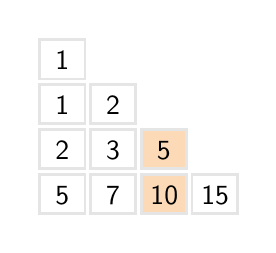
\begin{tikzpicture}
		\clip (0,0) rectangle(2.8,-2.5);
		\matrix[Matrix, anchor=north west] at (0,0) (M){ % Matrix contents  
			\sf 1 \\
			\sf 1 & \sf 2\\
			\sf 2 & \sf 3 & \sf 5\\
			\sf 5 & \sf 7 & \sf 10 & \sf 15\\
		};
		
		\begin{scope}[on background layer] 
			\node[DA,BurntOrange,fit=(M-3-3)(M-3-3)](subM){};
			\node[DA,BurntOrange,fit=(M-4-3)(M-4-3)](subM){};
		\end{scope}
	\end{tikzpicture}
	
\end{document}